\documentclass[11pt]{exam}
\usepackage[empty]{fullpage}
\usepackage{amsmath,amssymb}
\usepackage{colortbl}
\usepackage{subfig}
\usepackage{multicol}
\usepackage{tikz,pgfplots}
\usepgfplotslibrary{statistics}
\usepackage{color,comment,soul}

\newcommand{\blank}[1]{\underline{\hspace*{#1}}}
\newcommand{\ds}{\displaystyle}
\newcommand{\mymod}{~\mathrm{mod}~}


\begin{document}
\graphicspath{{/home/brian/Dropbox/HSC/Spring16/Math111/}}

\subsubsection*{Midterm 1 Review - Math 243}

\begin{questions}
%%%%%%%%%%%%%%%%%
%%% Problem 1 %%%
%%%%%%%%%%%%%%%%%
\question Consider the initial value problem
$$\frac{dy}{dt}-3(y-1)^{2/3}=0,~~~ y(0)=1$$
\begin{parts}
\item Verify that $y(t) = 1$ is a solution of the initial value problem above.  
\vfill

\item Verify that $y(t) = t^3+1$ is also a solution to the initial value problem.   
\vfill

\item Why doesn't this contradict the Uniqueness Theorem?  Explain. 
\vfill
\end{parts}
%%%%%%%%%%%%%%%%%
%%% Problem 2 %%%
%%%%%%%%%%%%%%%%%
\question Solve the initial value problem
$$y' = \frac{2t+1}{y^2}; \hspace{0.25in} y(1) = 2.$$ 
\vfill

\newpage
%%%%%%%%%%%%%%%%%
%%% Problem 3 %%%
%%%%%%%%%%%%%%%%%
\question Consider the equation 
$$\frac{dy}{dt} = (y-1)^2+t.$$ 
\begin{parts}
\item Sketch the slope field for this differential equation.  Just use the points $(t,y)$ with integer coordinates and $0 \leq t \leq 4$ and $0 \leq y \leq 4$. 

\begin{center}
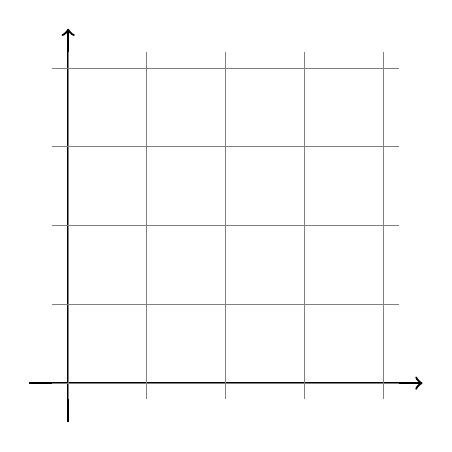
\begin{tikzpicture}
\draw[thick,->] (-0.5,0) -- (4.5,0);
\draw[thick,->] (0,-0.5) -- (0,4.5);
\draw[gray, thin] (-0.2,-0.2) grid (4.2,4.2);
\end{tikzpicture}
\end{center}

\item Use Euler's method with step size $\Delta t = 1$ to estimate the values of $y(t)$ for $t = 1, 2, 3$ given the initial condition $y(0) = 1$.  Add a sketch the Euler's method solution to the slope field above.  
\vfill
 



\end{parts}

%%%%%%%%%%%%%%%%%
%%% Problem 4 %%%
%%%%%%%%%%%%%%%%%
\question The following coupled system is a predator-prey population model.  
\begin{align*} 
\frac{dA}{dt} &= 5A - \frac{A^2}{1000} - 3AB \\[0.1in]
\frac{dB}{dt} &=  B \sqrt{A}
\end{align*}
\begin{parts}
\item Which of the variables $A$ or $B$ represents the predator and which represents the prey?  Explain your answer.  

\vfill
\item In the model, what would happen to the predator population if the prey is extinct?  
\vfill

\item What would happen to the prey population if there were no predators? 
\vfill

\end{parts}

\newpage
%%%%%%%%%%%%%%%%%
%%% Problem 5 %%%
%%%%%%%%%%%%%%%%%
\question Let $\ds{\frac{dy}{dt} = f_{\alpha}(y)}$ be a family of autonomous differential equations parametrized by $\alpha$ where $f_{\alpha}(y) = y^2-2y + \alpha$.
\begin{parts}
\item Draw phase lines for $\alpha = 0$, $\alpha = 1$, $\alpha = 2$.  In each case identify the equilibria and say whether they are stable, unstable, or nodes.   
\vfill

\item Use the phase lines in part (a) to sketch solutions to the initial value problem $y(0) =  0$ for the three cases, $\alpha = 0$, $\alpha=1$, and $\alpha =2$.  (Use a different graph for each $\alpha$).  
\vfill

\item What is (are) the bifurcation value(s) for this family of equations?  
\vfill
\item Draw the bifurcation diagram.  
\vfill 

\end{parts}
%%%%%%%%%%%%%%%%%
%%% Problem 6 %%%
%%%%%%%%%%%%%%%%%
\question Find the general solutions for the following differential equations.  
\begin{parts}
\item $\ds{\frac{dy}{dt} + \frac{2}{t}y = 4t^2.}$
\vfill
\item $\ds{\frac{dy}{dt} + 2y = 2t+1}$
\vfill

\end{parts}

\newpage

%%%%%%%%%%%%%%%%%
%%% Problem 7 %%%
%%%%%%%%%%%%%%%%%
\question Solve the following initial value problems. 
\begin{parts}
\part $y' - 5y = e^{5t}$, $y(0) = 4$. 
\begin{solution}
\end{solution}
\vfill

\part $\dfrac{dy}{dx} = x(y-1)$, $y(0) = 3$
\begin{solution}
$$y(t) = 2 e^{x^2/2} + 1.$$
\end{solution}
\vfill

\part $\dfrac{dy}{dt} + \dfrac{y}{t+1} = 6t$, $y(1) = 4$. 
\begin{solution}
$$y(t) = \dfrac{2t^3 + 3t^2 + 3}{t+1}.$$
\end{solution}
\vfill
\end{parts}

%%%%%%%%%%%%%%%%%
%%% Problem 8 %%%
%%%%%%%%%%%%%%%%%
\question Find the general solution to the partially coupled system
\begin{align*}
\dfrac{dx}{dt} &= 2x + 3y \\[0.1in]
\dfrac{dy}{dt} &= -4y.
\end{align*}
\vfill


%%%%%%%%%%%%%%%%%
%%% Problem 9 %%%
%%%%%%%%%%%%%%%%%
\question Suppose the population of fish in a pond obeys a logistic growth model $\dfrac{dP}{dt} = 0.3\left(1 - \dfrac{P}{2000} \right)$ where $t$ is measured in years.  
\begin{parts}
\part How would you change the model if 100 fish were harvested from the pond each year?
\vfill

\part How would you change the model if a quarter of the fish were harvested from the pond each year?
\vfill
\end{parts}


\newpage
%%%%%%%%%%%%%%%%%%
%%% Problem 10 %%%
%%%%%%%%%%%%%%%%%%
\question Consider the 2nd order homogeneous linear differential equation
$$y'' + 2y' + 5 y = 0.$$
\begin{parts}
\part Find the general solution. 

\vfill

\part Find the particular solution that satisfies the initial conditions $y(0) = 3$ and $y'(0) = 2$. 
\vfill

\end{parts}

\end{questions}

\end{document}
